This program will not have a graphical user interface or graphical representation of the results other than being able to export to bitmap. 

For simplicity, all cells can be allocated an integer from 0 to 9 and only one rule will apply. Adjacent cells can have a difference of at most 1, meaning cells surrounding a cell with state 8 can only has the value 7, 8 and 9. This also makes propagating the states faster since Manhattan distance can be used to limit the range of propagation.

\begin{figure}[!htb]
    \minipage{0.36\textwidth}
    \centering
    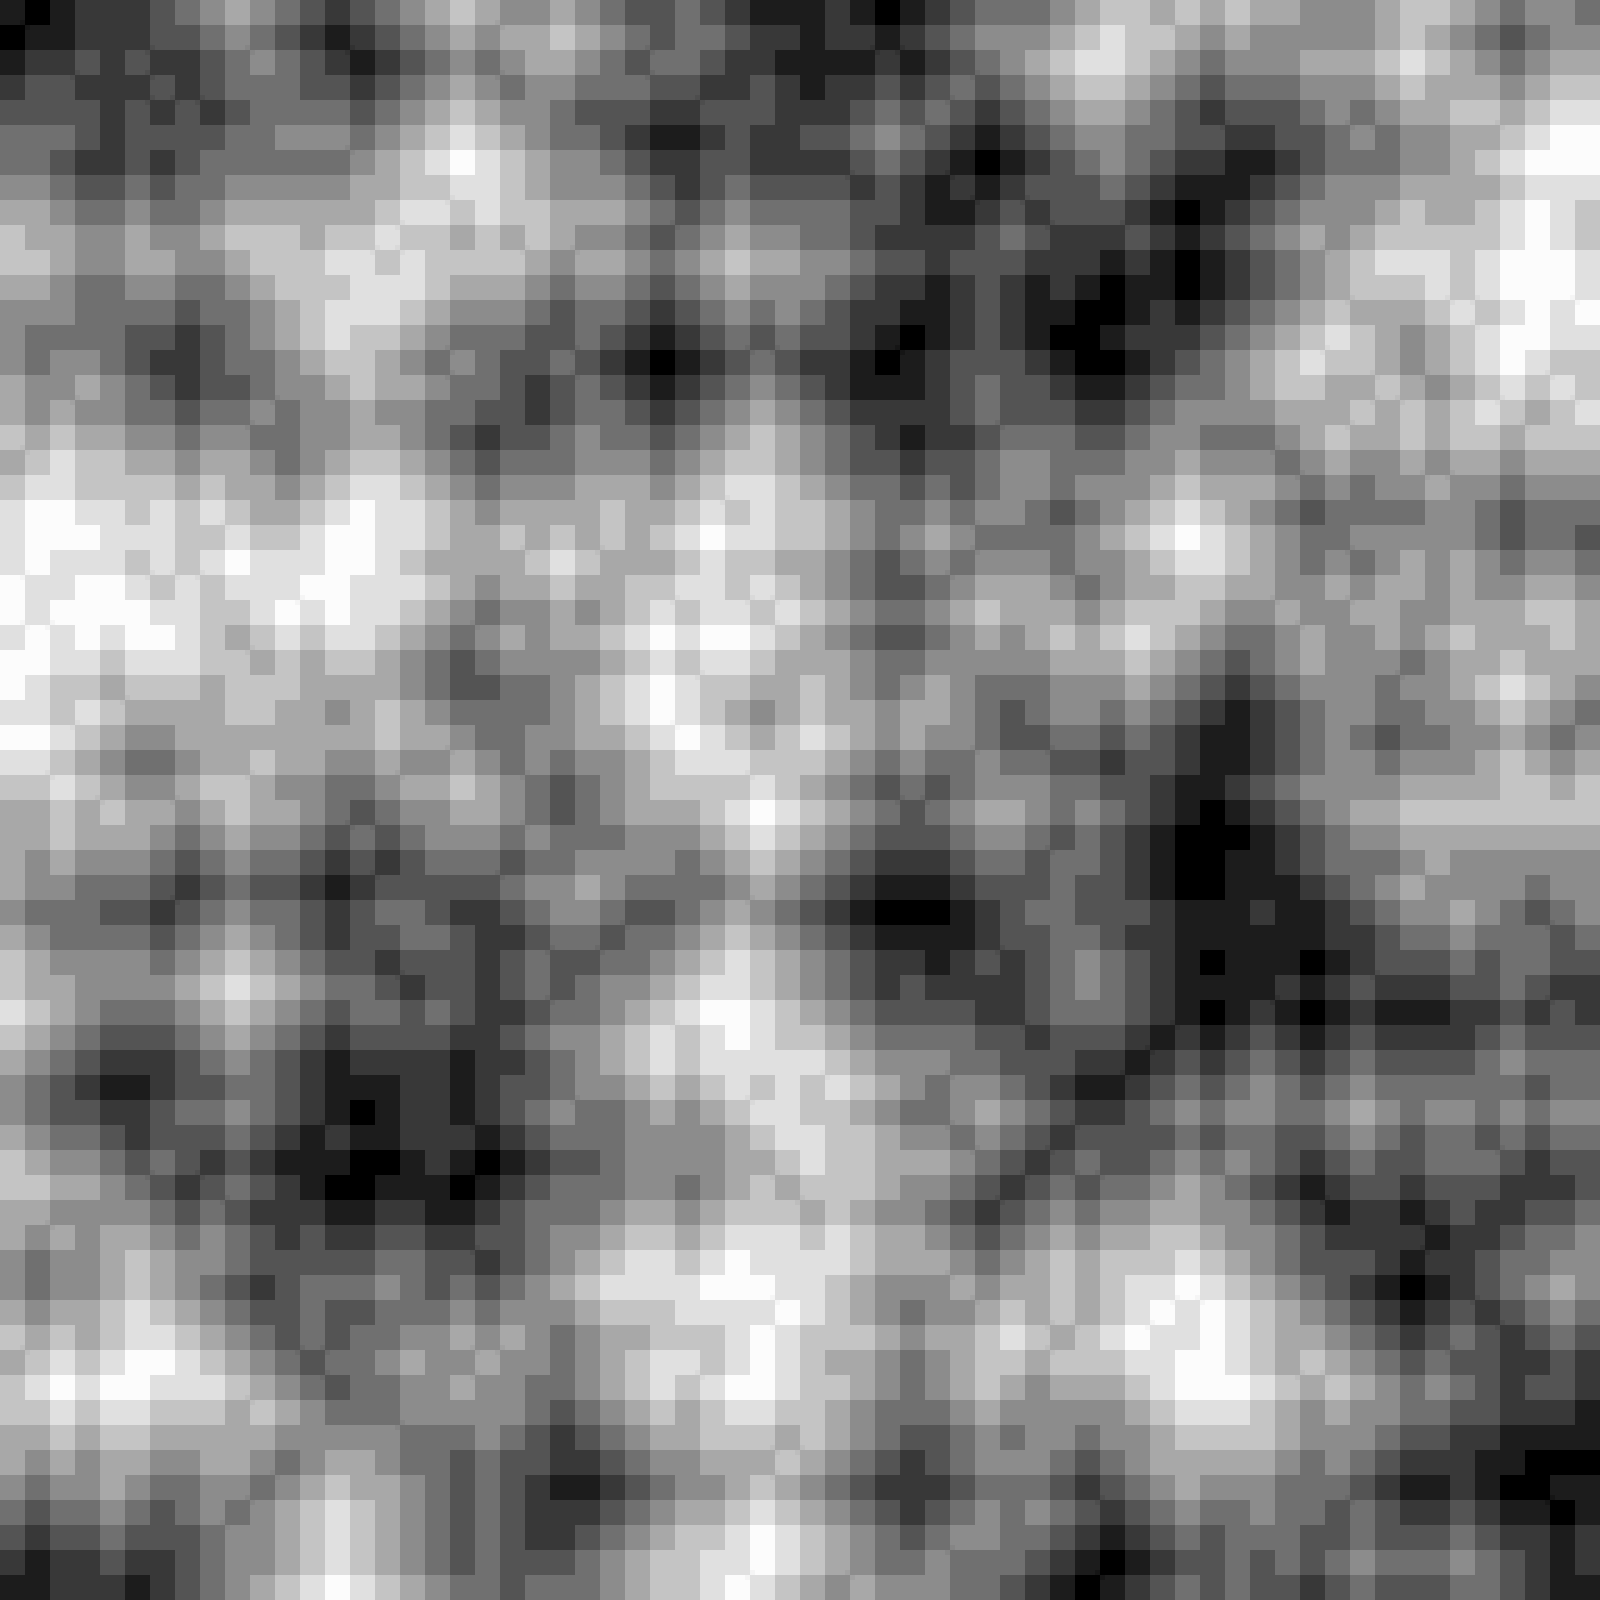
\includegraphics[height=6cm,keepaspectratio]{images/saved_result 64.png}
    \caption{Generated height map.}
    \endminipage\hfill
    \minipage{0.63\textwidth}
    \centering
    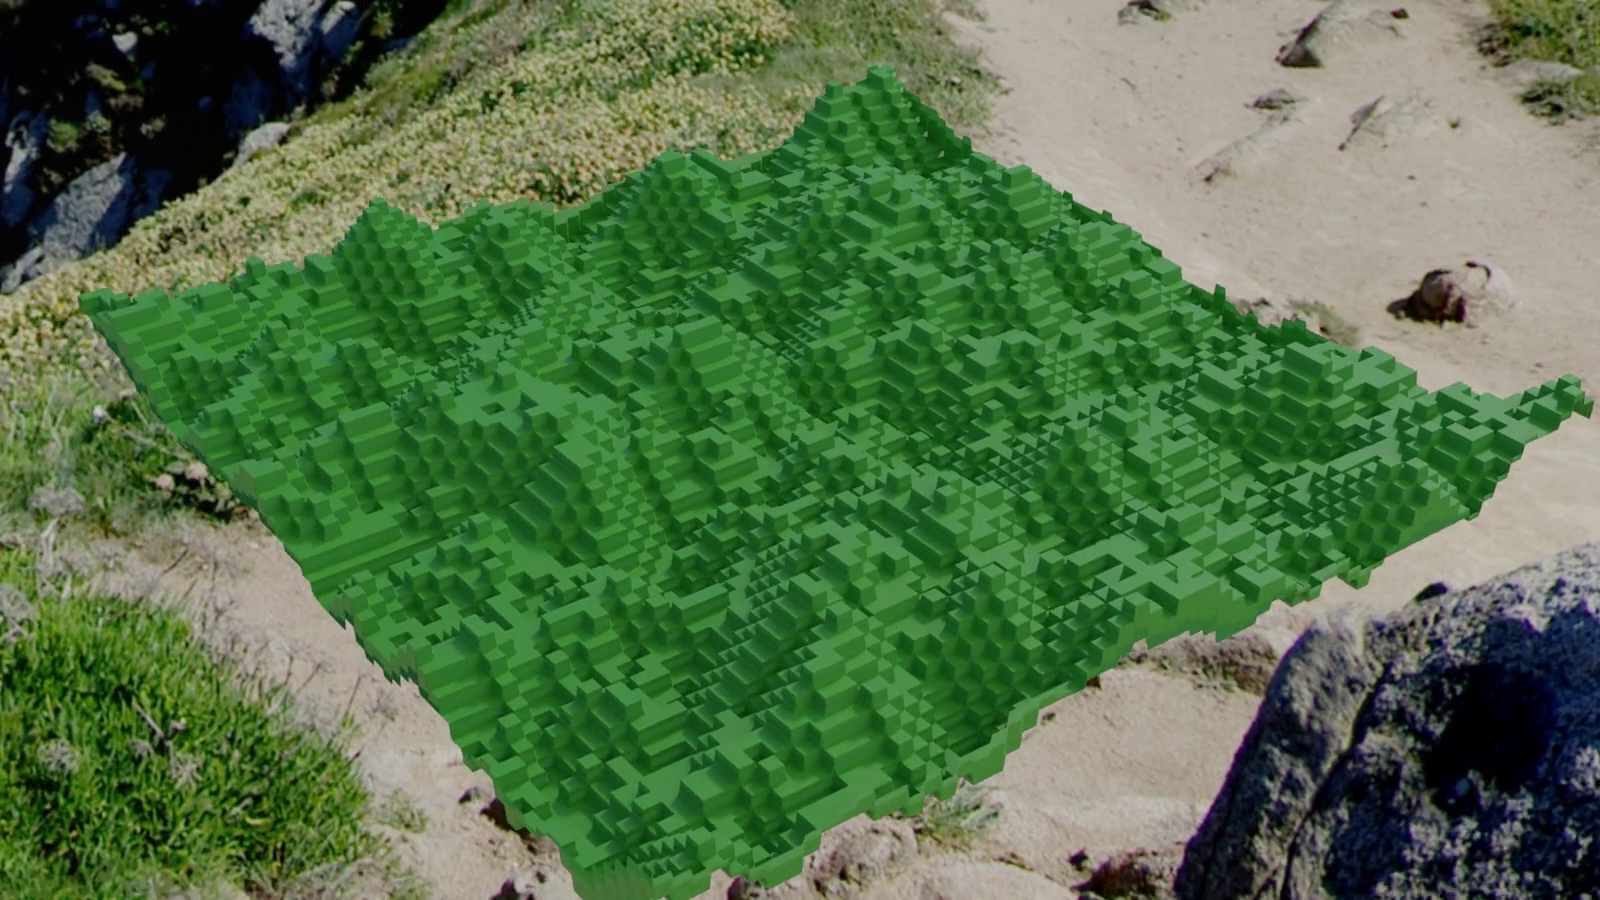
\includegraphics[height=6cm,keepaspectratio]{images/rendered_result_64.png}
    \caption{Generated terrain rendered in a 3D environment.}
    \endminipage\hfill
\end{figure}

    
This rule set simulates generation of mountain terrain in video games where no steep cliffs are present and the map has gradually changing attitudes. As can be seen in the images above, this algorithm aims to programmatically generate organic-seeming terrains.